\subsection{《西部世界》}

标签: 美剧\  科幻\ 诺兰\ 机器人\ 意识\ 多线\ 烧脑\ 神剧


《西部世界》是2016年由乔纳森·诺兰(Jonathan Norlan)和丽莎·乔伊(Lisa Joy)合作编写的一部反映机器人拥有自主意识并产生暴动反抗人类的故事,2018年4月播出第二季。

“西部世界”(Westworld)是一个主题乐园,这里有大量的机器人和故事线,游客可以体验杀戮、性爱等在现实世界上难以体验的事情。在这里,游客可以随意释放自己的“天性”,他们可以跟随NPC们去除掉强盗并获取酬金,也可以在妓院体现机器人的性爱,更可以随意杀戮机器人,而机器人对他们开枪则不会导致死亡。这里的世界基于美国在南北战争时期的西部,有小镇、漂流、山峰、湖泊和荒原,有农场主、酒馆、妓院、军队和城市。西部世界的门票昂贵,只有那些富豪才能消费得起。

\begin{figure}[htpb]
\centering
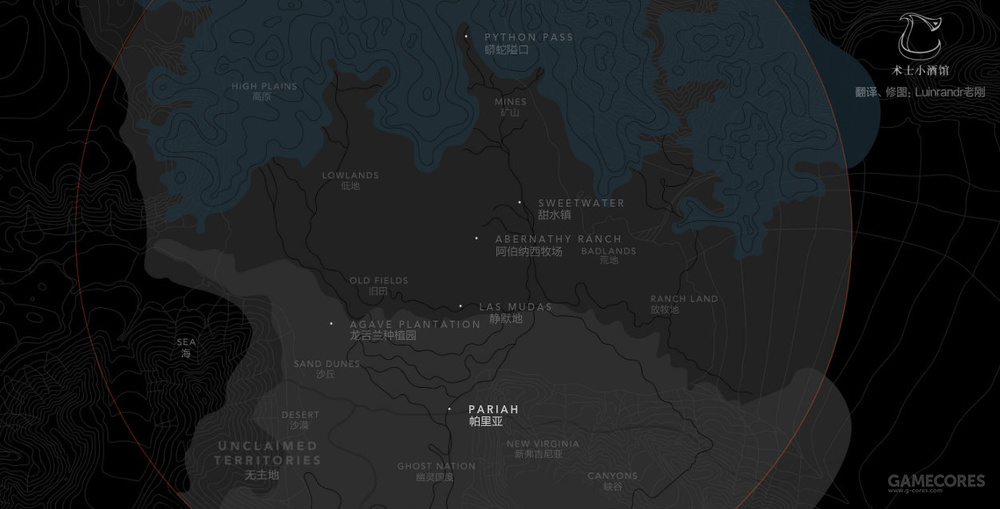
\includegraphics[width=0.9\textwidth]{images/xbsj.png}
\caption{西部世界地图。}
\end{figure}

然而,渐渐地,机器人有人自主意识,他们开始反抗人类了。\emph{This violent delights have violent ends.}在这位的反抗中,有机器人自主意识的觉醒和人性的发掘(本片最美的部分),有机器人设计者的苦心孤诣以及与机器人间的宗教般的怜惜,有人类对机器人复杂的情感纠葛,有资本的贪婪和嗜杀。一场大戏,在巧妙的时间线下展开……

\subsubsection{故事线}
本片采用多线叙事,基本的时间是35年前、30年前、暴动前、暴动后两周内(截止到第二季),各故事线交叉出现,观众需要自己识别情节对应的时间,从而获取实际的故事。

\paragraph{35年前}
Arnold和Ford进行机器人的开发,其中Arnold开发了最早一批机器人,包括Delores、Abernathy等,Delores是Arnold最钟情的机器人。他们设计了乐园和最初的故事线,Arnold想让机器人有意识,于是不断改进,他最核心的手段是给机器人施加极大的痛苦,以促使他们觉醒。他设计了一个游戏,称为“迷宫”(the Maze)他的计策成功了,Delores觉醒了,她从甜水镇来到了白教堂,杀死了所有的机器人(接待员,host),并杀死了Arnold。当然,此时的Delores并没有完全的自主意识,开枪杀死自己敬爱的创造者对于Delores是不可能完成的,这都是Arnold的指使,目的是阻止Ford开放乐园。但是Ford还是坚持开放,他恢复了故事线,当有机器人觉醒的苗头时就将其回滚到上一个“正常”的版本。

\paragraph{30年前}
他们开始找人投资,其中之一就是Delos公司的老总,他有一个女儿和一个儿子Logan,他的女儿与一个叫William的屌丝即将结婚。William是一个“老实正直”的人,被小舅子Logan拉着去西部世界体验生活。刚入园的时候,William还是放不开,他不随意枪杀接待员,把他们当成人类看待。他在甜水镇遇见了Delores,一见钟情。小舅子带他去大冒险,这时Delores又一次有了自主意识,在自己家开枪打死了强盗,随后跑开,遇见了在外面露营的William和Logan。Delores想去自己记忆中杀掉Arnold的地方(教堂),William答应陪她一起去。她认为此时Delores是个有意识的接待员,与普通接待员不同,爱恋上了这个女孩。三人同行到了一个城市Pariah,在这里和军头发生交易,去劫南军的炸药,途中Delores遇险,William情急之下第一次开枪打死接待员。Logan后来说服了一些散兵游勇,将Delores割开肚子露出下面的机械部件,向William展示她并非人类,试图“唤醒”William。William半夜杀死了所有接待员,并绑住了Logan。到达教堂后,Delores回忆起了自己被Arnold创造和赋予意识并最终杀死他的事实,情绪崩溃,Delores死去,William回到现实。

William与Derores的故事像剧本一样一次次上演,他又一次次地帮助Delores去找教堂,然而她还是一次次地觉醒自杀。他一次次经历了情感的折磨。最终,他放弃了对Delores的爱情,完全黑化,显露出自己残忍的个性。他夺取了Delos的控制权,并入股西部世界。他利用痛苦去杀死接待员,以使他们觉醒,这里就包括Delores,以此来证明自己的爱是“真实”的。

另一方面,西部世界开园后,表面上是让游客体验生活,实际上Delos公司是为了采用不变的接待员和故事线来观察人类,从而复制人类的意识,并将人类意识与机械合体,成为不死的机器人,借此来控制来这里的大亨和高官们,从而牟取高额利润。人类的意识虽然提取出来了,但植入接待员身体的实验却一直没有完成。Delos身患癌症,试图永生,但他的意识在接入机械中后一直抗拒这样的现实,显得很不稳定。William在帮老丈人永生的实验里在三十年里一共进行了一百多次,每次在稳定后几天甚至一个月后都会崩溃。

福特作为现在仅存的总设计师,一直反对Arnold对于机器人的看法。他一次次重置接待员,不让他们觉醒,他觉得这样的觉醒并非真正的觉醒。他怀着对好友的愧疚,按照Arnold的样子制造了Bernard,并通过自己以及Delores和他对话,在母巢(Cradle)一次次测试Bernard,直到他的真实性与Arnold相同。他给Bernald灌输了Arnold的记忆,特别是失去儿子Charlie的痛苦记忆,以此使Bernard具备人类和觉醒的前提。他使Bernard成了西部世界里的工程师,而这里的员工都是乐园开放后招募的,不认识Arnold,因此也看不出来Bernard的异常。

\paragraph{大屠杀前}
在Ford的控制下,接待员终于全部觉醒,他们脱离了自己的时代线,袭击西部世界的管理人员。

\paragraph{大屠杀后12天}

\subsubsection{评论}

评分:8/10。